% Options for packages loaded elsewhere
\PassOptionsToPackage{unicode}{hyperref}
\PassOptionsToPackage{hyphens}{url}
\PassOptionsToPackage{dvipsnames,svgnames,x11names}{xcolor}
\PassOptionsToPackage{space}{xeCJK}
\documentclass[
  10pt,
  a4paper,
]{article}
\usepackage{xcolor}
\usepackage[margin=22mm]{geometry}
\usepackage{amsmath,amssymb}
\setcounter{secnumdepth}{-\maxdimen} % remove section numbering
\usepackage{iftex}
\ifPDFTeX
  \usepackage[T1]{fontenc}
  \usepackage[utf8]{inputenc}
  \usepackage{textcomp} % provide euro and other symbols
\else % if luatex or xetex
  \usepackage{unicode-math} % this also loads fontspec
  \defaultfontfeatures{Scale=MatchLowercase}
  \defaultfontfeatures[\rmfamily]{Ligatures=TeX,Scale=1}
\fi
\usepackage{lmodern}
\ifPDFTeX\else
  % xetex/luatex font selection
  \ifXeTeX
    \usepackage{xeCJK}
    \setCJKmainfont[]{Hiragino Mincho ProN}
  \fi
  \ifLuaTeX
    \usepackage[]{luatexja-fontspec}
    \setmainjfont[]{Hiragino Mincho ProN}
  \fi
\fi
% Use upquote if available, for straight quotes in verbatim environments
\IfFileExists{upquote.sty}{\usepackage{upquote}}{}
\IfFileExists{microtype.sty}{% use microtype if available
  \usepackage[]{microtype}
  \UseMicrotypeSet[protrusion]{basicmath} % disable protrusion for tt fonts
}{}
\makeatletter
\@ifundefined{KOMAClassName}{% if non-KOMA class
  \IfFileExists{parskip.sty}{%
    \usepackage{parskip}
  }{% else
    \setlength{\parindent}{0pt}
    \setlength{\parskip}{6pt plus 2pt minus 1pt}}
}{% if KOMA class
  \KOMAoptions{parskip=half}}
\makeatother
\usepackage{longtable,booktabs,array}
\newcounter{none} % for unnumbered tables
\usepackage{calc} % for calculating minipage widths
% Correct order of tables after \paragraph or \subparagraph
\usepackage{etoolbox}
\makeatletter
\patchcmd\longtable{\par}{\if@noskipsec\mbox{}\fi\par}{}{}
\makeatother
% Allow footnotes in longtable head/foot
\IfFileExists{footnotehyper.sty}{\usepackage{footnotehyper}}{\usepackage{footnote}}
\makesavenoteenv{longtable}
\usepackage{graphicx}
\makeatletter
\newsavebox\pandoc@box
\newcommand*\pandocbounded[1]{% scales image to fit in text height/width
  \sbox\pandoc@box{#1}%
  \Gscale@div\@tempa{\textheight}{\dimexpr\ht\pandoc@box+\dp\pandoc@box\relax}%
  \Gscale@div\@tempb{\linewidth}{\wd\pandoc@box}%
  \ifdim\@tempb\p@<\@tempa\p@\let\@tempa\@tempb\fi% select the smaller of both
  \ifdim\@tempa\p@<\p@\scalebox{\@tempa}{\usebox\pandoc@box}%
  \else\usebox{\pandoc@box}%
  \fi%
}
% Set default figure placement to htbp
\def\fps@figure{htbp}
\makeatother
\setlength{\emergencystretch}{3em} % prevent overfull lines
\providecommand{\tightlist}{%
  \setlength{\itemsep}{0pt}\setlength{\parskip}{0pt}}
\usepackage{pdflscape}
\usepackage{bookmark}
\IfFileExists{xurl.sty}{\usepackage{xurl}}{} % add URL line breaks if available
\urlstyle{same}
\hypersetup{
  colorlinks=true,
  linkcolor={Maroon},
  filecolor={Maroon},
  citecolor={Blue},
  urlcolor={Blue},
  pdfcreator={LaTeX via pandoc}}

\author{}
\date{}

\begin{document}

\section{Three XYZ Directions Read from Complete Pairwise Relational
Waves}\label{three-xyz-directions-read-from-complete-pairwise-relational-waves}

\subsection{Growth of Internal Relational Directions and Saturation of
Spatial-Direction Readout in Closed AB, ABC, and ABCD
Systems}\label{growth-of-internal-relational-directions-and-saturation-of-spatial-direction-readout-in-closed-ab-abc-and-abcd-systems}

\textbf{Author:} Noriaki Kihara \textbf{ORCID:} 0009-0004-6753-4020
\textbf{Date:} July 20, 2026 \textbf{Version DOI:}
10.5281/zenodo.21454790 \textbf{Concept DOI:} 10.5281/zenodo.21454789
\textbf{Position:} ``Generative Structure of Dimensions'' series, Paper
2, v1

\begin{center}\rule{0.5\linewidth}{0.5pt}\end{center}

\subsection{Abstract}\label{abstract}

Previous closed two-body AB phase-system studies contained only one
phase-difference relation, \(AB\), and examined whether position and
acceleration-like readouts could be constructed from that
one-dimensional relation. They did not treat phase relations
corresponding to multiple spatial directions such as XY or XYZ. This
paper does not assume background coordinate axes in advance. Instead, it
examines whether relations readable as XY and XYZ directions can be
constructed from the complete pairwise relations of an ABC three-body
system and an ABCD four-body system.

For \(N\) bodies, define the set of all pairwise relations by

\[
\mathcal E_N
=
\bigl\{\{i,j\}\mid 1\le i<j\le N\bigr\},
\qquad
M=\lvert\mathcal E_N\rvert=\binom{N}{2}.
\]

One complex relational wave \(X_e\) is assigned to every relation
\(e\in\mathcal E_N\). All relational waves are physical state
components; neither C nor D is used as an observer. The state is
constructed to satisfy

\[
\sum_{e\in\mathcal E_N}X_e^2=R^2.
\]

Relations are coupled only when they share an endpoint. A real
skew-symmetric generator is built from these shared endpoints and phase
differences, and the system is evolved by the real orthogonal update
obtained from its Cayley transform.

In 32 trials of 720 steps for each configuration, AB had only one
relational wave and was stationary with generator rank zero. ABC had
three relational waves, \(AB\), \(BC\), and \(CA\), and all three were
active in every trial. Three directions readable internally as XYZ axes
emerged, but the generator rank was two: the phase relation actually
read out consisted of the two XY axes. The remaining Z direction was the
invariant normal determined by the XY plane and was not read out as an
independent phase relation. ABCD had six relational waves; in every
trial its generator had rank six, nullity zero, and decomposed into
three rotation planes. Of the six internal relational directions, the
three directions uniquely readable as spatial directions were XYZ, while
the remaining three had no unique direction.

Across all configurations, the maximum quadratic-closure error was
\(1.92\times10^{-13}\), the maximum drift of the absolute-square sum was
\(2.42\times10^{-13}\), and the maximum label-permutation covariance
error was \(1.47\times10^{-13}\). No stepwise state normalization,
observation damping, or absolute background axis was used.

This paper distinguishes the number of internal relational directions
from the number of directions uniquely readable as spatial directions.
ABC contains three directions internally, but only two phase axes, XY,
are read out. ABCD contains six directions internally, but only the
three XYZ axes are uniquely readable as spatial directions. This paper
interprets the additional relations introduced for five or more bodies
as non-uniquely oriented internal relations rather than new spatial
directions beyond XYZ. Identifying the remaining directions with
physical axes is outside the subject of this paper.

\begin{center}\rule{0.5\linewidth}{0.5pt}\end{center}

\subsection{0. Conclusion}\label{conclusion}

The previous AB two-body problem contained only one phase-difference
relation, \(AB\). Both position readout and acceleration-like readout
were constructed from this one-dimensional relation. The present work
extends the construction to the ABC three-body and ABCD four-body
problems and examines the readout of phase relations corresponding to
multiple spatial directions.

When complete pairwise relations are counted as independent state waves,
the number of internal relational directions is

\[
M=\binom{N}{2}.
\]

Therefore,

\[
AB:1,
\qquad
ABC:3,
\qquad
ABCD:6.
\]

ABC produces the three phase relations \(AB\), \(BC\), and \(CA\). These
can be read internally as three XYZ-axis directions. Its generator,
however, satisfies

\[
\operatorname{rank}K=2,
\qquad
\dim\ker K=1.
\]

The phase relation actually read out is therefore the pair of XY axes
corresponding to rank two. The remaining direction is the invariant
normal Z determined by the XY plane; it is not read out as an
independent phase relation.

Thus the ABC relation space decomposes as

\[
\boxed{
\text{one rotation plane}
\;\oplus\;
\text{one invariant direction}
}.
\]

In the numerical experiment, all three relational waves remained active
while this XY-plane/Z-normal structure, quadratic closure,
absolute-square sum, and label-permutation covariance were
simultaneously preserved.

ABCD produces six phase relations. Its generator satisfies

\[
\operatorname{rank}K=6,
\qquad
\dim\ker K=0,
\]

and the six directions decompose into three rotation planes. The six
internal relational directions cannot all be read as independent spatial
axes. The directions uniquely readable as spatial directions are the
three XYZ directions; the other three do not have uniquely determined
directions.

The central claim of this paper is therefore

\[
\boxed{
\text{internal relational directions increase, while}
\quad
\text{uniquely readable spatial directions stop at XYZ}
}.
\]

Increasing the number of complete pairwise relations for five or more
bodies does not add new uniquely readable spatial directions. This paper
reads the added relations as internal directions whose orientations are
not unique. The physical-axis identities of the residual directions are
outside the subject of this paper.

\begin{center}\rule{0.5\linewidth}{0.5pt}\end{center}

\subsection{1. Research Question}\label{research-question}

\subsubsection{1.1 Beginning with relations rather than background
coordinates}\label{beginning-with-relations-rather-than-background-coordinates}

One-, two-, and three-dimensional spaces are ordinarily described by the
number of coordinate axes specified in advance. Such a description
leaves the existence of those axes as a premise.

This paper reverses that order.

The initial objects are not spatial axes but relational waves between
bodies. Two bodies AB have one relation \(AB\). Three bodies ABC have
three relations \(AB\), \(BC\), and \(CA\). Four bodies ABCD have six
complete pairwise relations.

The question is:

\begin{quote}
When the system is extended from one AB relation to three ABC relations
and six ABCD relations, how many phase relations readable as XY and XYZ
directions can be determined uniquely?
\end{quote}

\subsubsection{1.2 The question left by the preceding AB
system}\label{the-question-left-by-the-preceding-ab-system}

The preceding closed two-body AB phase-system study showed that position
and acceleration-like harmonic readouts can be constructed from the
unlabeled two-body relation \(AB\) without assuming a background
coordinate system {[}2{]}.

The AB system, however, has only one phase-difference relation. The
preceding experiment therefore treated a one-dimensional relational
readout and did not treat multiple phase relations corresponding to XY
or XYZ directions.

The present work does not add a third observer wave. Instead, it treats
every pairwise relation of ABC and ABCD as a physical relational wave of
equal status.

\subsubsection{1.3 What is discriminated in this
paper}\label{what-is-discriminated-in-this-paper}

For each configuration, this paper determines:

\begin{enumerate}
\def\labelenumi{\arabic{enumi}.}
\tightlist
\item
  the number of complete pairwise relational waves;
\item
  the number of relational waves that are active;
\item
  whether the three ABC relations can distinguish the two XY axes and
  the Z normal;
\item
  whether the six ABCD relations can read out three XYZ directions
  uniquely;
\item
  whether an increase in internal relations also increases readable
  spatial directions;
\item
  whether quadratic closure and the absolute-square sum are preserved;
  and
\item
  whether the result transforms covariantly under permutations of body
  labels.
\end{enumerate}

\begin{center}\rule{0.5\linewidth}{0.5pt}\end{center}

\subsection{2. Classification of Claims}\label{classification-of-claims}

Definitions, mathematical consequences, numerical facts, physical
interpretations, and statements outside the subject are separated below.
The use of anonymity and quadratic closure follows the preceding Basic
Axiom System v4 {[}1{]}.

{\def\LTcaptype{none} % do not increment counter
\begin{landscape}
\begingroup\scriptsize
\begin{longtable}[]{@{}
  >{\raggedright\arraybackslash}p{(\linewidth - 4\tabcolsep) * \real{0.3333}}
  >{\raggedright\arraybackslash}p{(\linewidth - 4\tabcolsep) * \real{0.3333}}
  >{\raggedright\arraybackslash}p{(\linewidth - 4\tabcolsep) * \real{0.3333}}@{}}
\toprule\noalign{}
\begin{minipage}[b]{\linewidth}\raggedright
Object
\end{minipage} & \begin{minipage}[b]{\linewidth}\raggedright
Classification
\end{minipage} & \begin{minipage}[b]{\linewidth}\raggedright
Status in this paper
\end{minipage} \\
\midrule\noalign{}
\endhead
\bottomrule\noalign{}
\endlastfoot
No absolute physical meaning is assigned to a body label & Requirement
adopted from Axiom 0 & Tested by label-permutation covariance \\
\(\sum_e X_e^2=R^2\) & Closure condition & Computed at every step \\
Every pairwise relation is an independent relational wave & Model
definition & \(M=\binom{N}{2}\) \\
Only relations sharing an endpoint are coupled & Working hypothesis &
Implemented by relational adjacency \\
A real skew-symmetric generator is built from the sine of phase
differences & Working hypothesis & Not derived from Axioms 0 and 1
alone \\
A real skew-symmetric generator decomposes into two-dimensional rotation
blocks and a kernel & Mathematical consequence & Canonical form of a
real skew-symmetric matrix \\
A nonzero ABC generator has one rotation plane and a one-dimensional
kernel & Mathematical consequence & A nonzero \(3\times3\)
skew-symmetric matrix has rank two \\
All three ABC relational waves are active & Numerical fact & Verified in
32 trials \\
The ABCD generator has rank six & Numerical fact & Verified in 32
trials \\
Rank two in ABC is read as the two phase-readable XY axes &
Spatial-direction interpretation of this paper & Two phase axes are
actually read out \\
The one-dimensional ABC kernel is read as the Z normal &
Spatial-direction interpretation of this paper & Third direction
determined by the XY plane \\
The three ABCD rotation planes are read as XYZ & Spatial-direction
interpretation of this paper & Three of the six relations are read
uniquely \\
The remaining three ABCD directions & Spatial-direction interpretation
of this paper & Internal relations without unique direction \\
Directions added for five or more bodies & Generalized interpretation of
this paper & They increase non-unique internal directions, not XYZ \\
Physical-axis identities of the residual directions & Outside the
subject & Not identified here \\
\end{longtable}
\endgroup
\end{landscape}
}

\begin{center}\rule{0.5\linewidth}{0.5pt}\end{center}

\subsection{3. Complete Pairwise Relational-Wave
Model}\label{complete-pairwise-relational-wave-model}

\subsubsection{3.1 Relation set}\label{relation-set}

Consider \(N\) bodies. The letters A, B, C, and D are computational
identifiers and have no intrinsic physical roles.

Define

\[
\mathcal E_N
=
\bigl\{\{i,j\}\mid 1\le i<j\le N\bigr\}.
\]

The number of relations is

\[
M
=
\lvert\mathcal E_N\rvert
=
\binom{N}{2}
=
\frac{N(N-1)}{2}.
\]

The three configurations used in this paper are

\[
\begin{aligned}
\mathcal E_2&=\{AB\},\\
\mathcal E_3&=\{AB,BC,CA\},\\
\mathcal E_4&=\{AB,AC,AD,BC,BD,CD\}.
\end{aligned}
\]

Assign one complex state wave

\[
X_e=a_e+i b_e
\]

to every relation \(e\) and write the full state as

\[
X=
\begin{pmatrix}
X_{e_1} & X_{e_2} & \cdots & X_{e_M}
\end{pmatrix}^{\mathsf T}
\in\mathbb C^M.
\]

The relations \(AB\), \(BC\), \(CA\), and so on are not observation
channels. They are physical state components of equal status.

\begin{figure}
\centering
\pandocbounded{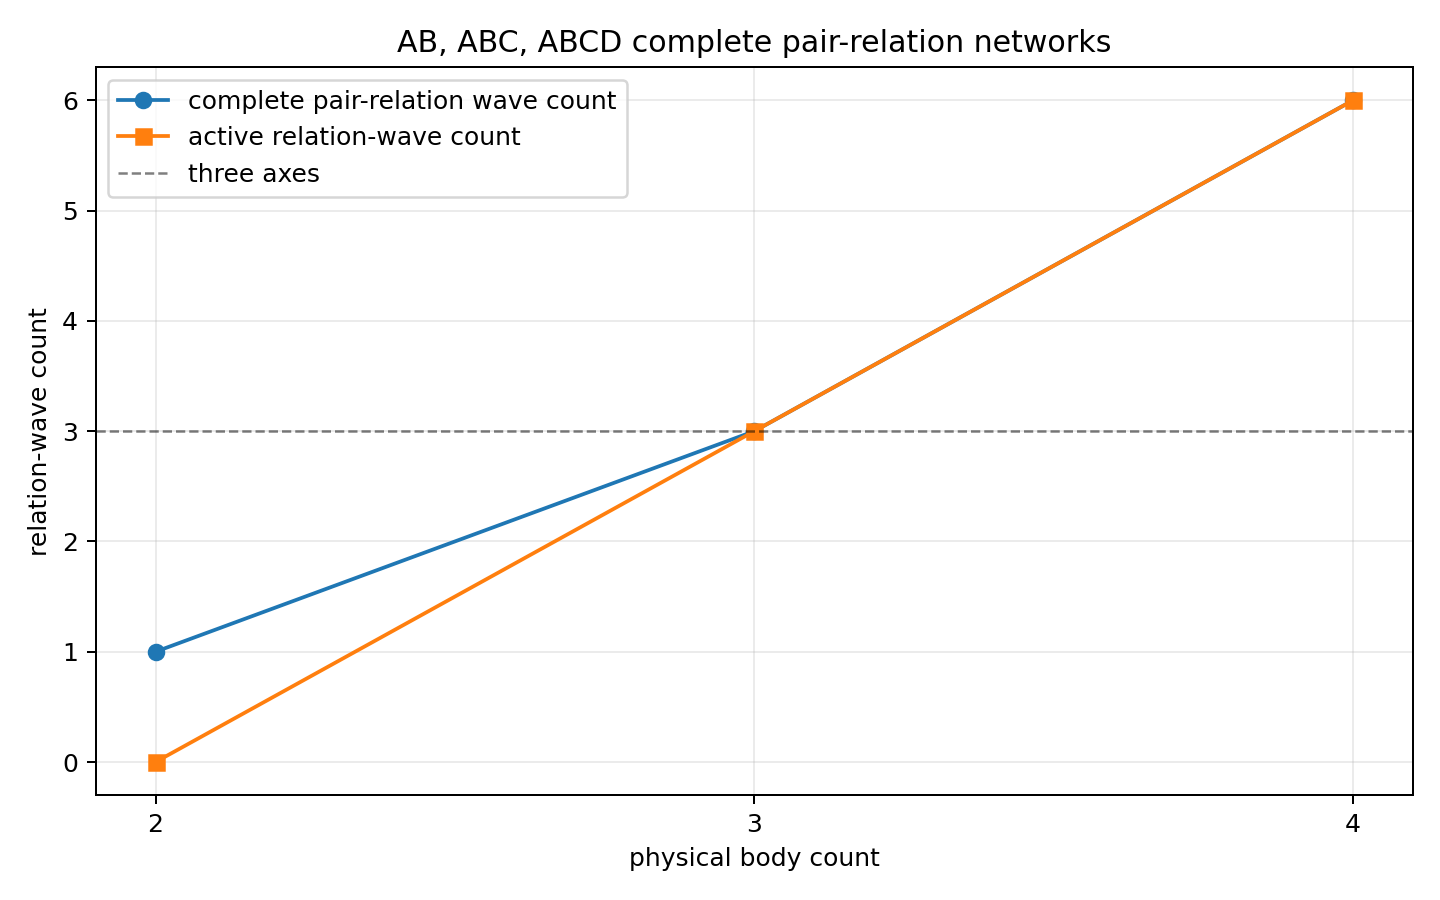
\includegraphics[keepaspectratio,alt={Number of complete pairwise relational waves}]{figures/complete_pair_relation_wave_count_v1.png}}
\caption{Number of complete pairwise relational waves}
\end{figure}

\subsubsection{3.2 Adjacency between
relations}\label{adjacency-between-relations}

Two distinct relations \(e,f\in\mathcal E_N\) are adjacent only when
they share one endpoint:

\[
A_{ef}
=
\begin{cases}
1,
& e\ne f\ \text{and}\ e\cap f\ne\varnothing,\\
0,
& \text{otherwise}.
\end{cases}
\]

This is the line-graph construction of the complete graph \(K_N\), where
bodies are vertices and pairwise relations are edges {[}3{]}.

The coupling is therefore determined not by the body names but only by
whether two relations share an endpoint.

\begin{center}\rule{0.5\linewidth}{0.5pt}\end{center}

\subsection{4. Quadratic Closure and Initial
State}\label{quadratic-closure-and-initial-state}

\subsubsection{4.1 Closure condition}\label{closure-condition}

Define the quadratic closure of the complex relational waves by

\[
q(X)
=
X^{\mathsf T}X
=
\sum_{e\in\mathcal E_N}X_e^2
=
R^2.
\]

This is the equivalent form of zero-square-sum closure obtained by
writing the closure term as

\[
(iR)^2=-R^2
\]

in

\[
\sum_{e\in\mathcal E_N}X_e^2+(iR)^2=0.
\]

The numerical experiment directly preserves the rearranged form
\(q(X)=R^2\).

For \(X_e=a_e+i b_e\), write

\[
q(X)=E+iF,
\]

where

\[
E
=
\sum_e\left(a_e^2-b_e^2\right)
\]

and

\[
F
=
2\sum_e a_e b_e.
\]

At every step, the experiment directly tests

\[
E=R^2,
\qquad
F=0.
\]

An independent comparison quantity is the absolute-square sum

\[
H(X)
=
X^\dagger X
=
\sum_e\lvert X_e\rvert^2
=
\sum_e\left(a_e^2+b_e^2\right).
\]

The quantities \(q(X)\) and \(H(X)\) are not the same. The first is the
sum of complex squares; the second is the sum of absolute squares.

\subsubsection{4.2 Initial closed state}\label{initial-closed-state}

For \(M>1\), construct real unit vectors \(u,v\in\mathbb R^M\)
satisfying

\[
u^{\mathsf T}u=1,
\qquad
v^{\mathsf T}v=1,
\qquad
u^{\mathsf T}v=0.
\]

The initial state is

\[
X(0)
=
\sqrt{R^2+s^2}\,u
+
i s\,v,
\]

where \(s\) is the initial imaginary amplitude. Then

\[
\begin{aligned}
X(0)^{\mathsf T}X(0)
&=
(R^2+s^2)u^{\mathsf T}u
-s^2v^{\mathsf T}v
+2is\sqrt{R^2+s^2}\,u^{\mathsf T}v\\
&=R^2.
\end{aligned}
\]

Thus closure holds exactly at the initial state.

The experiment uses

\[
R^2=1,
\qquad
s=0.35.
\]

For AB, where \(M=1\),

\[
X_{AB}(0)=R.
\]

\begin{center}\rule{0.5\linewidth}{0.5pt}\end{center}

\subsection{5. Closure-Preserving
Generator}\label{closure-preserving-generator}

\subsubsection{5.1 Skew-symmetric generator from phase
differences}\label{skew-symmetric-generator-from-phase-differences}

Let the initial phase of a relational wave be

\[
\theta_e=\arg X_e(0).
\]

Define the unnormalized generator coupling only endpoint-sharing
relations by

\[
\widetilde K_{ef}
=
A_{ef}\sin(\theta_f-\theta_e).
\]

Because \(A_{ef}=A_{fe}\) and

\[
\sin(\theta_e-\theta_f)
=
-\sin(\theta_f-\theta_e),
\]

we have

\[
\widetilde K^{\mathsf T}
=
-\widetilde K.
\]

When nonzero, it is normalized by its spectral norm:

\[
K
=
\frac{\widetilde K}{\lVert\widetilde K\rVert_2}.
\]

This generator is constructed solely from relational sharing and phase
differences. The particular sine-coupling rule is not derived from Axiom
0 and quadratic closure in the preceding Basic Axiom System v4 {[}1{]}.
It is the closure-preserving working hypothesis used in this
constructive numerical experiment.

\subsubsection{5.2 Cayley update}\label{cayley-update}

For a real skew-symmetric generator \(K\), define the one-step update by

\[
U
=
\left(I-\gamma K\right)^{-1}
\left(I+\gamma K\right),
\]

where \(\gamma\) is a real coefficient determining the finite update
width.

The Cayley transform of a real skew-symmetric matrix is real orthogonal
{[}5{]}:

\[
U^{\mathsf T}U=I.
\]

The state update is

\[
X_{s+1}=UX_s.
\]

\subsubsection{5.3 Two conserved
quantities}\label{two-conserved-quantities}

Because \(U\) is real orthogonal, the complex bilinear quadratic form
satisfies

\[
\begin{aligned}
q(X_{s+1})
&=
(UX_s)^{\mathsf T}(UX_s)\\
&=
X_s^{\mathsf T}U^{\mathsf T}UX_s\\
&=
X_s^{\mathsf T}X_s\\
&=q(X_s).
\end{aligned}
\]

Since \(U^\dagger=U^{\mathsf T}\), the absolute-square sum is also
conserved:

\[
\begin{aligned}
H(X_{s+1})
&=
(UX_s)^\dagger(UX_s)\\
&=
X_s^\dagger U^{\mathsf T}UX_s\\
&=
X_s^\dagger X_s\\
&=H(X_s).
\end{aligned}
\]

These quantities are not preserved by renormalizing the state at every
step. They are preserved by the orthogonality of the update itself.

\begin{center}\rule{0.5\linewidth}{0.5pt}\end{center}

\subsection{6. Rotation Planes and Spatial-Direction
Readout}\label{rotation-planes-and-spatial-direction-readout}

\subsubsection{6.1 Canonical form of a real skew-symmetric
matrix}\label{canonical-form-of-a-real-skew-symmetric-matrix}

A real skew-symmetric matrix \(K\in\mathbb R^{M\times M}\) can be
decomposed by a real orthogonal matrix \(Q\) into two-dimensional
rotation blocks and a zero block {[}4{]}:

\[
Q^{\mathsf T}KQ
=
\bigoplus_{j=1}^{r}
\begin{pmatrix}
0 & -\sigma_j\\
\sigma_j & 0
\end{pmatrix}
\oplus
0_{M-2r},
\qquad
\sigma_j>0.
\]

Hence

\[
\operatorname{rank}K=2r
\]

is always even, and

\[
\dim\ker K=M-2r.
\]

Here \(r\) is the number of independent rotation planes, and \(\ker K\)
is the set of invariant directions not moved by the generator.

\subsubsection{6.2 AB}\label{ab}

For AB, \(M=1\), and there is no other relation with which the single
relation can mix. Therefore,

\[
K=(0),
\qquad
\operatorname{rank}K=0,
\qquad
\dim\ker K=1.
\]

There is one invariant direction but no rotation plane. AB alone cannot
construct a plane together with a normal to that plane.

\subsubsection{6.3 ABC}\label{abc}

For ABC,

\[
X=
\begin{pmatrix}
X_{AB} & X_{BC} & X_{CA}
\end{pmatrix}^{\mathsf T}
\in\mathbb C^3.
\]

The rank of a nonzero \(3\times3\) real skew-symmetric matrix is even
and does not exceed three. Consequently,

\[
\operatorname{rank}K=2,
\qquad
\dim\ker K=1.
\]

The ABC relation space decomposes as

\[
\mathbb R^3
=
\mathcal P_{\mathrm{rot}}
\oplus
\ker K,
\]

with

\[
\dim\mathcal P_{\mathrm{rot}}=2,
\qquad
\dim\ker K=1.
\]

Once a nonzero generator exists, the three relational directions contain
one rotation plane and one invariant direction. This paper reads the
rotation plane as the two phase-readable XY axes and the invariant
direction as the Z normal determined by the XY plane. ABC contains three
XYZ directions internally, but the independent phase relation readout is
limited to the two XY axes.

\begin{figure}
\centering
\pandocbounded{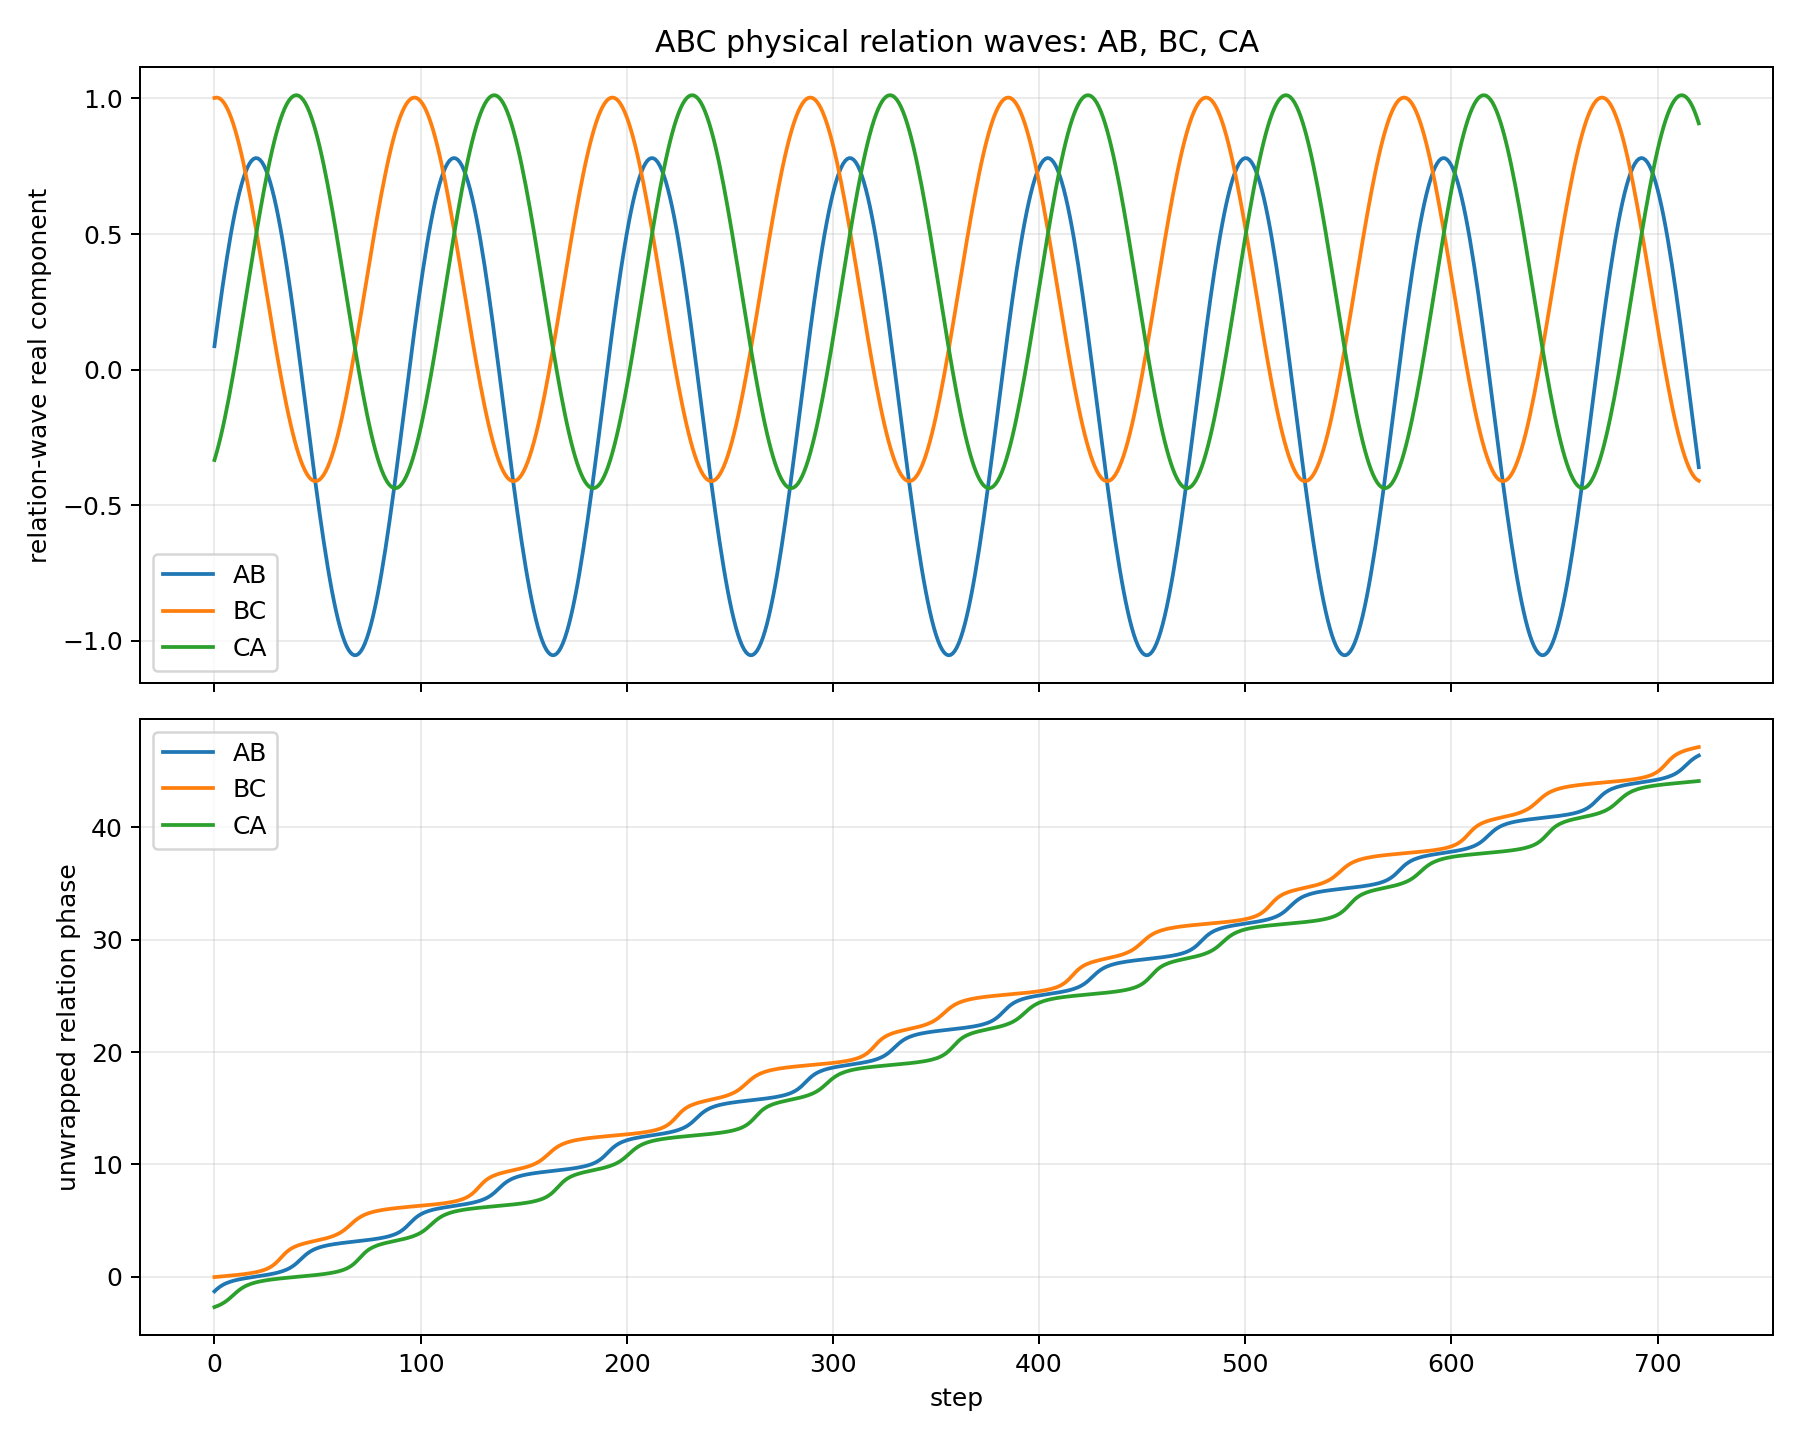
\includegraphics[keepaspectratio,alt={Three ABC relational waves}]{figures/ABC_three_physical_relation_waves_v1.png}}
\caption{Three ABC relational waves}
\end{figure}

\subsubsection{6.4 Invariant projection}\label{invariant-projection}

Let \(P_0\) be the orthogonal projector onto \(\ker K\). Then

\[
KP_0=P_0K=0.
\]

For the Cayley update,

\[
UP_0=P_0U=P_0.
\]

Therefore,

\[
P_0X_{s+1}
=
P_0UX_s
=
P_0X_s,
\]

and the kernel component is conserved.

Because \(\ker K\) is one-dimensional in ABC, this conserved component
determines a unique Z direction up to sign. Z is not an independent
phase-relation readout; it is the normal determined by the XY plane.

\subsubsection{6.5 ABCD}\label{abcd}

For ABCD, \(M=6\). The rank of a real skew-symmetric generator can be

\[
0,2,4,6.
\]

In all 32 trials,

\[
\operatorname{rank}K=6,
\qquad
\dim\ker K=0,
\]

so

\[
r=3.
\]

ABCD therefore has six active relational directions that decompose into
three rotation planes. This paper reads these three rotation planes as
the XYZ directional readout. The remaining three internal directions
depend on phase selection within the rotation planes and do not
determine unique spatial directions.

\begin{figure}
\centering
\pandocbounded{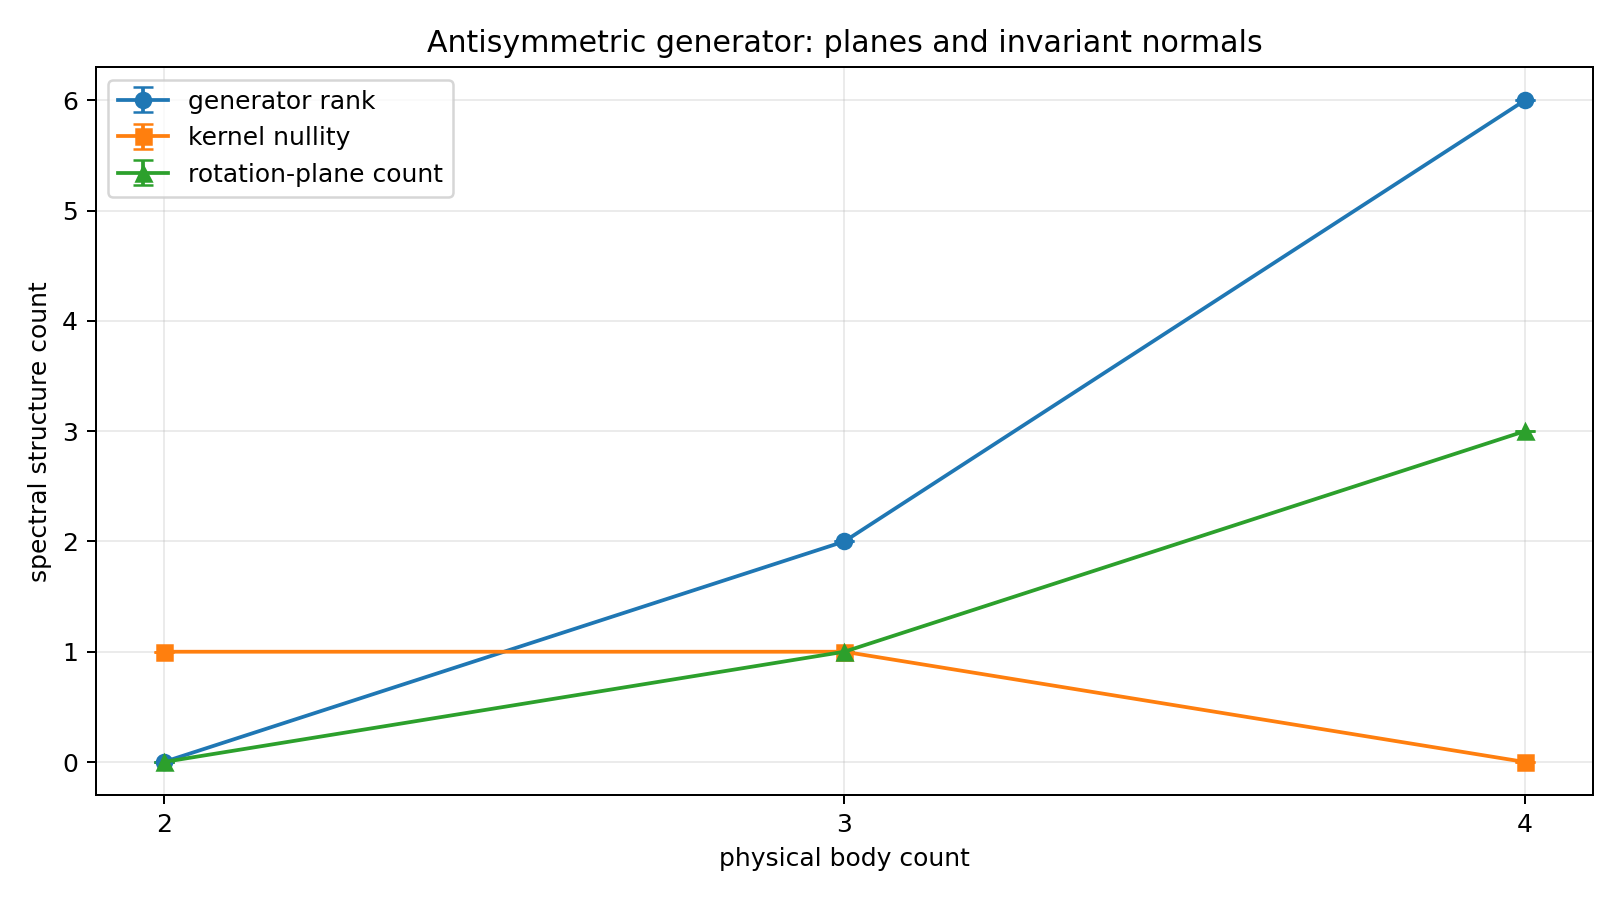
\includegraphics[keepaspectratio,alt={Generator plane and invariant-direction structure}]{figures/generator_plane_normal_structure_v1.png}}
\caption{Generator plane and invariant-direction structure}
\end{figure}

\begin{center}\rule{0.5\linewidth}{0.5pt}\end{center}

\subsection{7. Label-Permutation
Covariance}\label{label-permutation-covariance}

\subsubsection{7.1 Permutation action}\label{permutation-action}

Let \(\pi\) be a permutation of body labels and \(P_\pi\) the induced
permutation matrix on the relational-wave space. The initial state
transforms as

\[
X'_0=P_\pi X_0.
\]

Compatibility with anonymity requires

\[
K'=P_\pi K P_\pi^{\mathsf T},
\]

\[
U'=P_\pi U P_\pi^{\mathsf T},
\]

and therefore

\[
X'_s=P_\pi X_s
\]

for the complete trajectory.

\subsubsection{7.2 Meaning of the test}\label{meaning-of-the-test}

The test verifies that relabeling A, B, C, and D changes only the
component ordering of the same physical state. The implementation
contains no privileged rule tied to a particular body name.

For ABC, the kernel projector is also tested for

\[
P'_0
=
P_\pi P_0P_\pi^{\mathsf T}
\]

within numerical precision.

\begin{center}\rule{0.5\linewidth}{0.5pt}\end{center}

\subsection{8. Numerical Experiment}\label{numerical-experiment}

\subsubsection{8.1 Conditions}\label{conditions}

{\def\LTcaptype{none} % do not increment counter
\begingroup\scriptsize
\begin{longtable}[]{@{}lr@{}}
\toprule\noalign{}
Item & Value \\
\midrule\noalign{}
\endhead
\bottomrule\noalign{}
\endlastfoot
Configurations & AB, ABC, ABCD \\
Trials & 32 for each configuration \\
Update steps & 720 for each trial \\
\(R^2\) & 1.0 \\
Initial imaginary amplitude \(s\) & 0.35 \\
Random seed & 20260720 \\
Invariant tolerance & \(10^{-10}\) \\
Covariance tolerance & \(10^{-10}\) \\
Activity-variance threshold & \(10^{-10}\) \\
Stepwise state normalization & None \\
Observation damping & None \\
Observer-only C or D & None \\
Absolute background axis & None \\
\end{longtable}
\endgroup
}

\subsubsection{8.2 Quantities recorded at every
step}\label{quantities-recorded-at-every-step}

For each state \(X_s\), the experiment records

\[
E_s
=
\sum_e
\left[
(\Re X_{e,s})^2
-(\Im X_{e,s})^2
\right],
\]

\[
F_s
=
2\sum_e
(\Re X_{e,s})(\Im X_{e,s}),
\]

\[
\varepsilon_{q,s}
=
\sqrt{(E_s-R^2)^2+F_s^2},
\]

and

\[
H_s
=
\sum_e\lvert X_{e,s}\rvert^2.
\]

The computation also records generator rank, kernel dimension, number of
rotation planes, number of independent rotation frequencies, activity
variance of each relational wave, kernel-projection drift, and
covariance errors of the generator, update matrix, and trajectory after
label permutation.

\subsubsection{8.3 Acceptance conditions}\label{acceptance-conditions}

The experiment requires all of the following:

\begin{enumerate}
\def\labelenumi{\arabic{enumi}.}
\tightlist
\item
  quadratic-closure error is below tolerance;
\item
  absolute-square-sum drift is below tolerance;
\item
  update-matrix orthogonality error is below tolerance;
\item
  the generator, update matrix, and trajectory are covariant after label
  permutation;
\item
  all three ABC relational waves are active;
\item
  ABC has one rotation plane and a one-dimensional kernel;
\item
  the ABC kernel projection is conserved; and
\item
  activity and spectral structure are recorded for all six ABCD
  relational waves.
\end{enumerate}

\begin{center}\rule{0.5\linewidth}{0.5pt}\end{center}

\subsection{9. Results}\label{results}

\subsubsection{9.1 Main results by
configuration}\label{main-results-by-configuration}

{\def\LTcaptype{none} % do not increment counter
\begingroup\scriptsize
\begin{longtable}[]{@{}
  >{\raggedright\arraybackslash}p{(\linewidth - 12\tabcolsep) * \real{0.1111}}
  >{\raggedleft\arraybackslash}p{(\linewidth - 12\tabcolsep) * \real{0.1481}}
  >{\raggedleft\arraybackslash}p{(\linewidth - 12\tabcolsep) * \real{0.1481}}
  >{\raggedleft\arraybackslash}p{(\linewidth - 12\tabcolsep) * \real{0.1481}}
  >{\raggedleft\arraybackslash}p{(\linewidth - 12\tabcolsep) * \real{0.1481}}
  >{\raggedleft\arraybackslash}p{(\linewidth - 12\tabcolsep) * \real{0.1481}}
  >{\raggedleft\arraybackslash}p{(\linewidth - 12\tabcolsep) * \real{0.1481}}@{}}
\toprule\noalign{}
\begin{minipage}[b]{\linewidth}\raggedright
Configuration
\end{minipage} & \begin{minipage}[b]{\linewidth}\raggedleft
Relational waves
\end{minipage} & \begin{minipage}[b]{\linewidth}\raggedleft
Active waves
\end{minipage} & \begin{minipage}[b]{\linewidth}\raggedleft
Generator rank
\end{minipage} & \begin{minipage}[b]{\linewidth}\raggedleft
Kernel dimension
\end{minipage} & \begin{minipage}[b]{\linewidth}\raggedleft
Rotation planes
\end{minipage} & \begin{minipage}[b]{\linewidth}\raggedleft
Independent frequencies
\end{minipage} \\
\midrule\noalign{}
\endhead
\bottomrule\noalign{}
\endlastfoot
AB & 1 & 0 & 0 & 1 & 0 & 0 \\
ABC & 3 & 3 & 2 & 1 & 1 & 1 \\
ABCD & 6 & 6 & 6 & 0 & 3 & 3 \\
\end{longtable}
\endgroup
}

Every entry in the table was the same in all 32 trials of the
corresponding configuration.

\subsubsection{9.2 Conserved quantities and
covariance}\label{conserved-quantities-and-covariance}

{\def\LTcaptype{none} % do not increment counter
\begingroup\scriptsize
\begin{longtable}[]{@{}
  >{\raggedright\arraybackslash}p{(\linewidth - 8\tabcolsep) * \real{0.1579}}
  >{\raggedleft\arraybackslash}p{(\linewidth - 8\tabcolsep) * \real{0.2105}}
  >{\raggedleft\arraybackslash}p{(\linewidth - 8\tabcolsep) * \real{0.2105}}
  >{\raggedleft\arraybackslash}p{(\linewidth - 8\tabcolsep) * \real{0.2105}}
  >{\raggedleft\arraybackslash}p{(\linewidth - 8\tabcolsep) * \real{0.2105}}@{}}
\toprule\noalign{}
\begin{minipage}[b]{\linewidth}\raggedright
Configuration
\end{minipage} & \begin{minipage}[b]{\linewidth}\raggedleft
Maximum closure error
\end{minipage} & \begin{minipage}[b]{\linewidth}\raggedleft
Maximum absolute-square drift
\end{minipage} & \begin{minipage}[b]{\linewidth}\raggedleft
Maximum orthogonality error
\end{minipage} & \begin{minipage}[b]{\linewidth}\raggedleft
Maximum trajectory-covariance error
\end{minipage} \\
\midrule\noalign{}
\endhead
\bottomrule\noalign{}
\endlastfoot
AB & \(0\) & \(0\) & \(0\) & \(0\) \\
ABC & \(1.3628\times10^{-13}\) & \(1.6809\times10^{-13}\) &
\(5.0984\times10^{-16}\) & \(1.1776\times10^{-13}\) \\
ABCD & \(1.9218\times10^{-13}\) & \(2.4114\times10^{-13}\) &
\(8.7433\times10^{-16}\) & \(1.4609\times10^{-13}\) \\
\end{longtable}
\endgroup
}

Across all configurations,

\[
\max_s\lvert q(X_s)-R^2\rvert
=
1.9218001973240896\times10^{-13},
\]

\[
\max_s\lvert H(X_s)-H(X_0)\rvert
=
2.41140440948584\times10^{-13},
\]

and

\[
\varepsilon_{\mathrm{label,max}}
=
1.4608516699761366\times10^{-13}.
\]

All values are below the tolerance \(10^{-10}\).

\begin{figure}
\centering
\pandocbounded{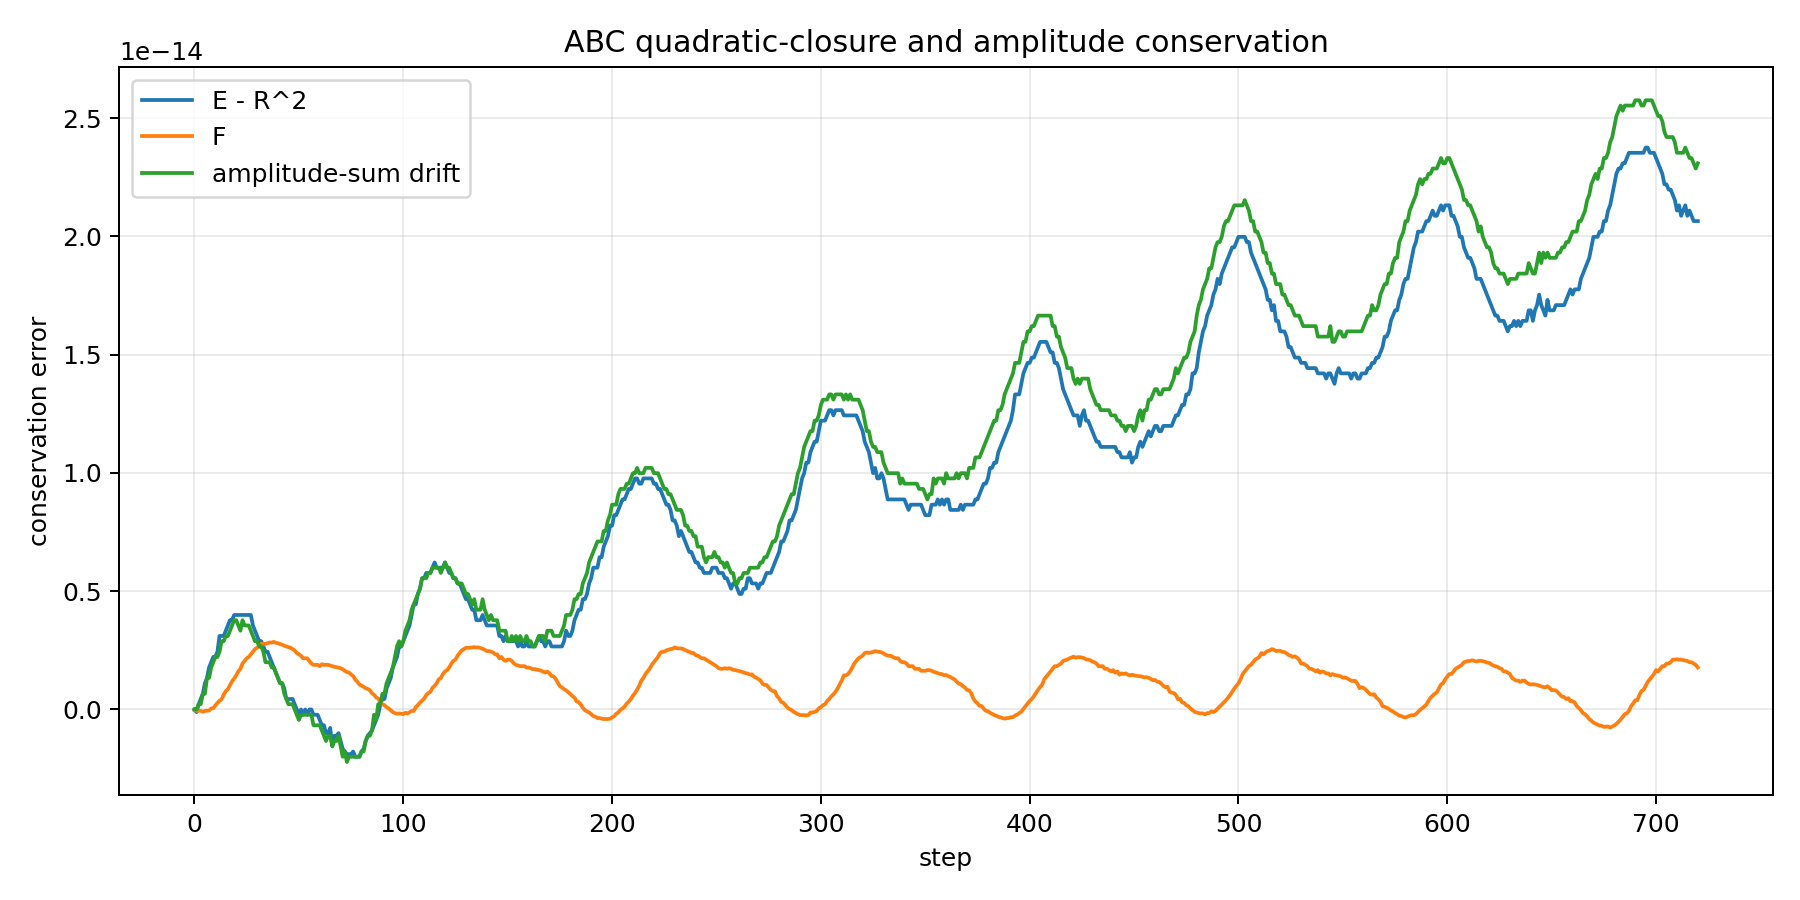
\includegraphics[keepaspectratio,alt={ABC conservation}]{figures/ABC_relation_wave_conservation_v1.png}}
\caption{ABC conservation}
\end{figure}

\subsubsection{9.3 AB result}\label{ab-result}

AB has only one relational wave, \(AB\). Since there is no separate
relation sharing an endpoint with it, the generator is zero and the
state is stationary in all 32 trials.

A single relation cannot generate an internal rotation of relational
space.

\subsubsection{9.4 ABC result}\label{abc-result}

ABC has three relational waves, \(AB\), \(BC\), and \(CA\), and all
three are active in all 32 trials. The ABC relation space therefore
contains three directions readable internally as XYZ axes.

In every trial,

\[
\operatorname{rank}K=2,
\qquad
\dim\ker K=1.
\]

The state decomposes into one rotation plane and one invariant
direction. The rank-two rotation plane is the pair of XY axes actually
read out as a phase relation. The one-dimensional kernel is the Z normal
determined by the XY plane and is not read out as an independent phase
relation.

The maximum kernel-projection drift is

\[
4.073028073875021\times10^{-14},
\]

the maximum drift of the squared kernel-projection norm is

\[
4.718447854656915\times10^{-14},
\]

and the maximum drift of the squared active-plane norm is

\[
1.34781075189494\times10^{-13}.
\]

The maximum label-permutation covariance error of the kernel projector
is

\[
7.591035761743328\times10^{-16}.
\]

Thus the Z normal is not fixed to a particular label. It is determined
covariantly from the XY phase relation and the generator.

\begin{figure}
\centering
\pandocbounded{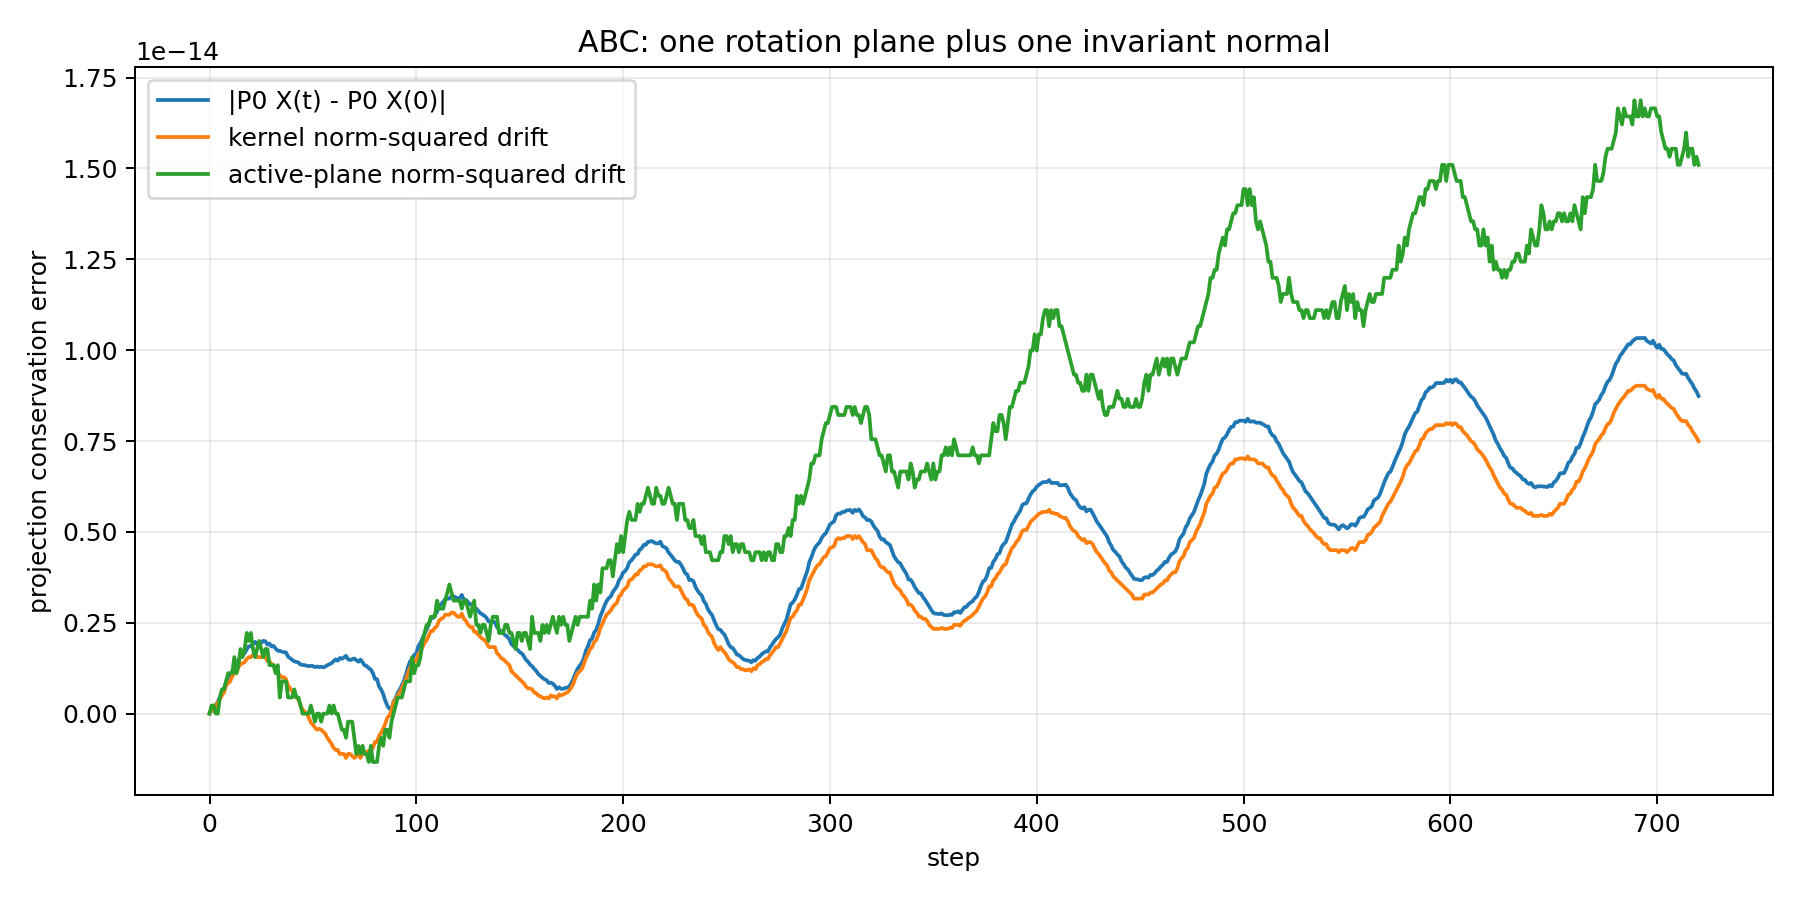
\includegraphics[keepaspectratio,alt={Conservation of the ABC plane and normal}]{figures/ABC_one_plane_one_normal_conservation_v1.png}}
\caption{Conservation of the ABC plane and normal}
\end{figure}

\subsubsection{9.5 ABCD result}\label{abcd-result}

ABCD has six complete pairwise relational waves, and all six are active
in all 32 trials. The ABCD relation space therefore contains six
internal relational directions.

In every trial,

\[
\operatorname{rank}K=6,
\qquad
\dim\ker K=0.
\]

The motion decomposes into three rotation planes distinguished as three
independent rotation frequencies. This paper reads the three rotation
planes as the XYZ directional readout.

Of the six internal relational directions, the uniquely readable spatial
directions are XYZ. The other three depend on phase selection within the
rotation planes and do not determine unique spatial directions. ABCD
therefore increases the number of internal relational directions to six
while the number of readable spatial directions stops at XYZ.

\begin{center}\rule{0.5\linewidth}{0.5pt}\end{center}

\subsection{10. Discussion}\label{discussion}

\subsubsection{10.1 Why ABC is the minimum
configuration}\label{why-abc-is-the-minimum-configuration}

AB has only one relational direction and cannot construct a rotation
plane.

ABC has three complete pairwise relations. A nonzero three-dimensional
real skew-symmetric generator decomposes into one two-dimensional
rotation plane and one one-dimensional kernel.

Thus ABC is the minimum complete pairwise relational system having

\[
\boxed{
\text{three internal XYZ directions}
=
\text{two readable XY axes}
+
\text{a Z normal determined by the XY plane}
}.
\]

The third direction is not an absolute axis specified in advance. It is
the kernel of the generator acting on the three relational directions
and is determined by its relation to the rotation plane.

\subsubsection{10.2 A right angle is not specified in
advance}\label{a-right-angle-is-not-specified-in-advance}

The model does not first specify an orthogonal XYZ coordinate system and
then define a rotation.

The initial objects are three relational waves and a skew-symmetric
generator that mixes them. The two-dimensional rotation subspace
\(\mathcal P_{\mathrm{rot}}\) and the kernel \(\ker K\) are orthogonal
under the real inner product:

\[
\mathcal P_{\mathrm{rot}}
\perp
\ker K.
\]

The orthogonal relation is therefore obtained from the decomposition of
relational motion rather than specified as a background spatial
relation. Orthogonality in this model means orthogonality under the real
inner product of relational-wave space.

\subsubsection{10.3 Internal relational directions and spatial-direction
readout}\label{internal-relational-directions-and-spatial-direction-readout}

The number of internal relational directions is not the same as the
number of directions uniquely readable as spatial directions.

{\def\LTcaptype{none} % do not increment counter
\begingroup\scriptsize
\begin{longtable}[]{@{}
  >{\raggedright\arraybackslash}p{(\linewidth - 6\tabcolsep) * \real{0.2308}}
  >{\raggedleft\arraybackslash}p{(\linewidth - 6\tabcolsep) * \real{0.3077}}
  >{\raggedright\arraybackslash}p{(\linewidth - 6\tabcolsep) * \real{0.2308}}
  >{\raggedright\arraybackslash}p{(\linewidth - 6\tabcolsep) * \real{0.2308}}@{}}
\toprule\noalign{}
\begin{minipage}[b]{\linewidth}\raggedright
Configuration
\end{minipage} & \begin{minipage}[b]{\linewidth}\raggedleft
Internal relational directions
\end{minipage} & \begin{minipage}[b]{\linewidth}\raggedright
Phase-relation readout
\end{minipage} & \begin{minipage}[b]{\linewidth}\raggedright
Spatial-direction readout
\end{minipage} \\
\midrule\noalign{}
\endhead
\bottomrule\noalign{}
\endlastfoot
AB & 1 & One \(AB\) relation & One-dimensional \\
ABC & 3 & Two XY axes & XY axes and the Z normal determined by them \\
ABCD & 6 & Three rotation planes & Three XYZ axes \\
\end{longtable}
\endgroup
}

ABC contains three relational directions, but the phase-relation readout
consists of the two XY axes. The third direction Z is the normal
determined by the XY plane and is not an independent phase relation.

ABCD contains six relational directions, but they do not become six
spatial axes. They decompose into three rotation planes, and the
uniquely readable spatial directions are XYZ. The remaining three do not
have uniquely determined directions.

\subsubsection{10.4 XYZ becomes readable with four
bodies}\label{xyz-becomes-readable-with-four-bodies}

AB reads one relation. ABC reads the two-axis XY phase relation and
determines the Z normal from it. ABCD produces three rotation planes and
reads the three XYZ directions uniquely as spatial directions.

Therefore, a relation structure readable as the three spatial XYZ
directions becomes available in the ABCD four-body system.

\subsubsection{10.5 What increases beyond four
bodies}\label{what-increases-beyond-four-bodies}

For five or more bodies, the number of complete pairwise relations

\[
M=\binom{N}{2}
\]

continues to grow. These added relations do not define new unique
spatial axes. This paper interprets the increase as additional internal
relations without unique direction; the spatial-direction readout does
not exceed XYZ.

The physical-axis identities of the residual directions are outside the
subject of this paper.

\begin{center}\rule{0.5\linewidth}{0.5pt}\end{center}

\subsection{11. Scope of the Claims}\label{scope-of-the-claims}

\subsubsection{11.1 Facts verified by the numerical
experiment}\label{facts-verified-by-the-numerical-experiment}

\begin{enumerate}
\def\labelenumi{\arabic{enumi}.}
\tightlist
\item
  Complete pairwise relations of AB, ABC, and ABCD were implemented as
  physical waves of equal status without observer-only waves.
\item
  The numbers of internal relational directions were one for AB, three
  for ABC, and six for ABCD.
\item
  All three ABC relational waves were active in every trial, and the
  generator had rank two and kernel dimension one.
\item
  All six ABCD relational waves were active in every trial, and the
  rank-six, zero-kernel generator decomposed into three rotation planes
  with three independent rotation frequencies.
\item
  Quadratic closure and the absolute-square sum were preserved without
  stepwise state normalization.
\item
  The generator, update matrix, trajectory, and kernel projection were
  covariant under label permutations.
\end{enumerate}

\subsubsection{11.2 Spatial-direction interpretation adopted in this
paper}\label{spatial-direction-interpretation-adopted-in-this-paper}

\begin{enumerate}
\def\labelenumi{\arabic{enumi}.}
\tightlist
\item
  The one AB relation is a one-dimensional phase readout.
\item
  Rank two in ABC is the two-axis XY phase readout.
\item
  The one-dimensional ABC kernel is the Z normal determined by the XY
  plane.
\item
  The three ABCD rotation planes are the three XYZ directional readouts.
\item
  The remaining three ABCD directions are internal relations without
  unique direction.
\item
  Directions added for five or more bodies increase internal relations
  without adding spatial directions beyond XYZ.
\end{enumerate}

\subsubsection{11.3 Items not fixed in this
paper}\label{items-not-fixed-in-this-paper}

The numerical experiment covers AB, ABC, and ABCD. The statement for
five or more bodies is the generalized spatial-direction interpretation
of this paper.

The phase-difference sine generator is the closure-preserving working
hypothesis of the model.

This paper does not assign physical-axis identities to residual
directions that are not uniquely readable as spatial directions.

\begin{center}\rule{0.5\linewidth}{0.5pt}\end{center}

\subsection{12. Reproducibility}\label{reproducibility}

The numerical results are based on the following program:

\resizebox{\linewidth}{!}{\texttt{次元の生成構造/対照実験\_一角度円周位相調和読出し\_v1/run\_ab\_abc\_abcd\_complete\_pair\_relation\_network\_preliminary\_v1.py}}

The principal outputs are:

\begin{itemize}
\tightlist
\item
  ab\_abc\_abcd\_complete\_pair\_relation\_network\_preliminary\_result\_v1.json
\item
  ab\_abc\_abcd\_complete\_pair\_relation\_network\_trial\_summary\_v1.csv
\item
  ab\_abc\_abcd\_complete\_pair\_relation\_network\_body\_summary\_v1.csv
\item
  ab\_abc\_abcd\_complete\_pair\_relation\_network\_selected\_series\_v1.csv
\item
  ab\_abc\_abcd\_complete\_pair\_relation\_network\_preliminary\_report\_v1.md
\end{itemize}

They are stored in:

\resizebox{\linewidth}{!}{\texttt{次元の生成構造/対照実験\_一角度円周位相調和読出し\_v1/ab\_abc\_abcd\_complete\_pair\_relation\_network\_preliminary\_result\_v1/}}

\begin{center}\rule{0.5\linewidth}{0.5pt}\end{center}

\subsection{13. Final Conclusion}\label{final-conclusion}

The previous AB two-body problem had only one phase-difference relation,
\(AB\), and constructed position and acceleration-like readouts as
one-dimensional relational readouts.

The present work extends the model to the ABC three-body and ABCD
four-body problems and constructs relations readable as XY and XYZ
directions from complete pairwise phase differences.

Without specifying background spatial axes in advance, the number of
internal relational directions grows as

\[
1\longrightarrow3\longrightarrow6.
\]

In ABC, all three relational waves are active while the skew-symmetric
generator decomposes as

\[
\text{one rotation plane}
\oplus
\text{one invariant direction}.
\]

ABC therefore contains three XYZ directions internally, but the phase
relation actually read out consists of the two XY axes. Z is the normal
determined by the XY plane and is not read out as an independent phase
relation.

In ABCD, six relational waves decompose into three rotation planes. This
paper reads the three rotation planes as the XYZ directional readout. Of
the six internal relational directions, the remaining three have no
uniquely determined directions.

Extending the system to five or more bodies increases the number of
internal relational directions but does not increase the number of
uniquely readable spatial directions. What increases is the number of
internal relations without unique direction.

Therefore,

\[
\boxed{
\text{internal relational directions increase, while}
\quad
\text{uniquely readable spatial directions stop at XYZ}
}.
\]

The physical-axis identities of the residual directions are outside the
subject of this paper.

\begin{center}\rule{0.5\linewidth}{0.5pt}\end{center}

\subsection{References}\label{references}

\subsubsection{Author's related works}\label{authors-related-works}

\begin{enumerate}
\def\labelenumi{\arabic{enumi}.}
\tightlist
\item
  Noriaki Kihara, ``Basic Axiom System of the Unnamed Equal-Amplitude
  Composite-Wave Model, v4,'' Zenodo, 2026. Version DOI:
  \href{https://doi.org/10.5281/zenodo.21316620}{10.5281/zenodo.21316620},
  Concept DOI:
  \href{https://doi.org/10.5281/zenodo.21315735}{10.5281/zenodo.21315735}.
\item
  Noriaki Kihara, ``Preliminary Summary of Harmonic Readout and c=1 Area
  Sweep in an AB Two-Body Closed Phase System, v4,'' Zenodo, 2026.
  Version DOI:
  \href{https://doi.org/10.5281/zenodo.21374317}{10.5281/zenodo.21374317},
  Concept DOI:
  \href{https://doi.org/10.5281/zenodo.21318696}{10.5281/zenodo.21318696}.
\end{enumerate}

\subsubsection{External references}\label{external-references}

\begin{enumerate}
\def\labelenumi{\arabic{enumi}.}
\setcounter{enumi}{2}
\tightlist
\item
  Hassler Whitney, ``Congruent Graphs and the Connectivity of Graphs,''
  \emph{American Journal of Mathematics}, 54(1), 150--168, 1932. DOI:
  \href{https://doi.org/10.2307/2371086}{10.2307/2371086}.
\item
  Milan Vujivčić, Fedor Herbut, and Gradimir Vujivčić, ``Canonical Form
  for Matrices Under Unitary Congruence Transformations. I:
  Conjugate-Normal Matrices,'' \emph{SIAM Journal on Applied
  Mathematics}, 23(2), 225--238, 1972. DOI:
  \href{https://doi.org/10.1137/0123025}{10.1137/0123025}.
\item
  Fasma Diele, Luciano Lopez, and R. Peluso, ``The Cayley Transform in
  the Numerical Solution of Unitary Differential Systems,''
  \emph{Advances in Computational Mathematics}, 8(4), 317--334, 1998.
  DOI:
  \href{https://doi.org/10.1023/A:1018908700358}{10.1023/A:1018908700358}.
\end{enumerate}

\end{document}
